\chapter{Design einer Datenbank}


%============================

\section{Domino Designer 8.5}
\label{sec:4designelemente}

In diesem Kapitel werden der Domino-Designer, die \textit{Tools} und die Elemente, die dieser bereitstellt, behandelt. Es werden
jedoch \textit{nicht} alle verfügbaren Elemente angeführt, sondern lediglich diese Design-Elemente  
welche notwendig sind, um das geforderte Template (Kapitel 3.4) zu erstellen. 
Für weitere Design-Elemente wird auf Fachliteratur verwiesen.\newline
\newline
Die Abbildungen 3.1 und 3.2 zeigen die Benutzeroberfläche des Domino-Designers.  
\begin{figure}[H]
    \centerline{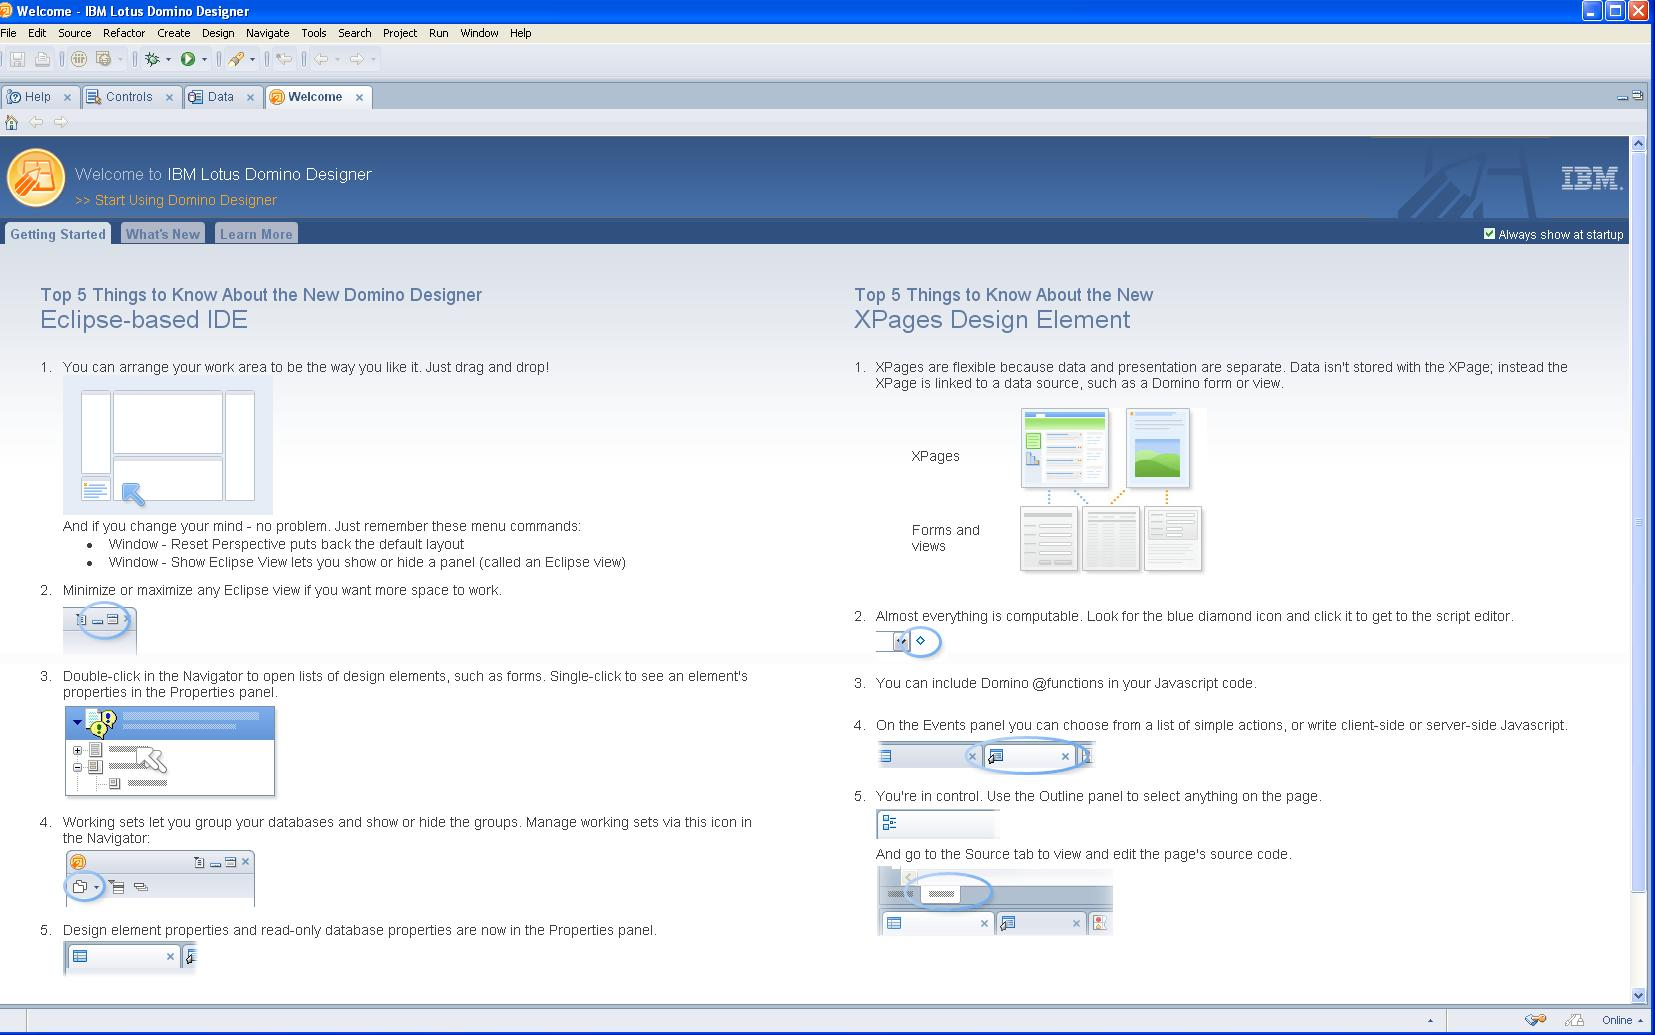
\includegraphics[scale=0.35]{pics/startansicht_designer}}
    \caption[Domino-Designer]{\label{FiG:Domino-Designer}
	Startansicht Domino-Designer 8.5}
\end{figure}

\begin{figure}[H]
    \centerline{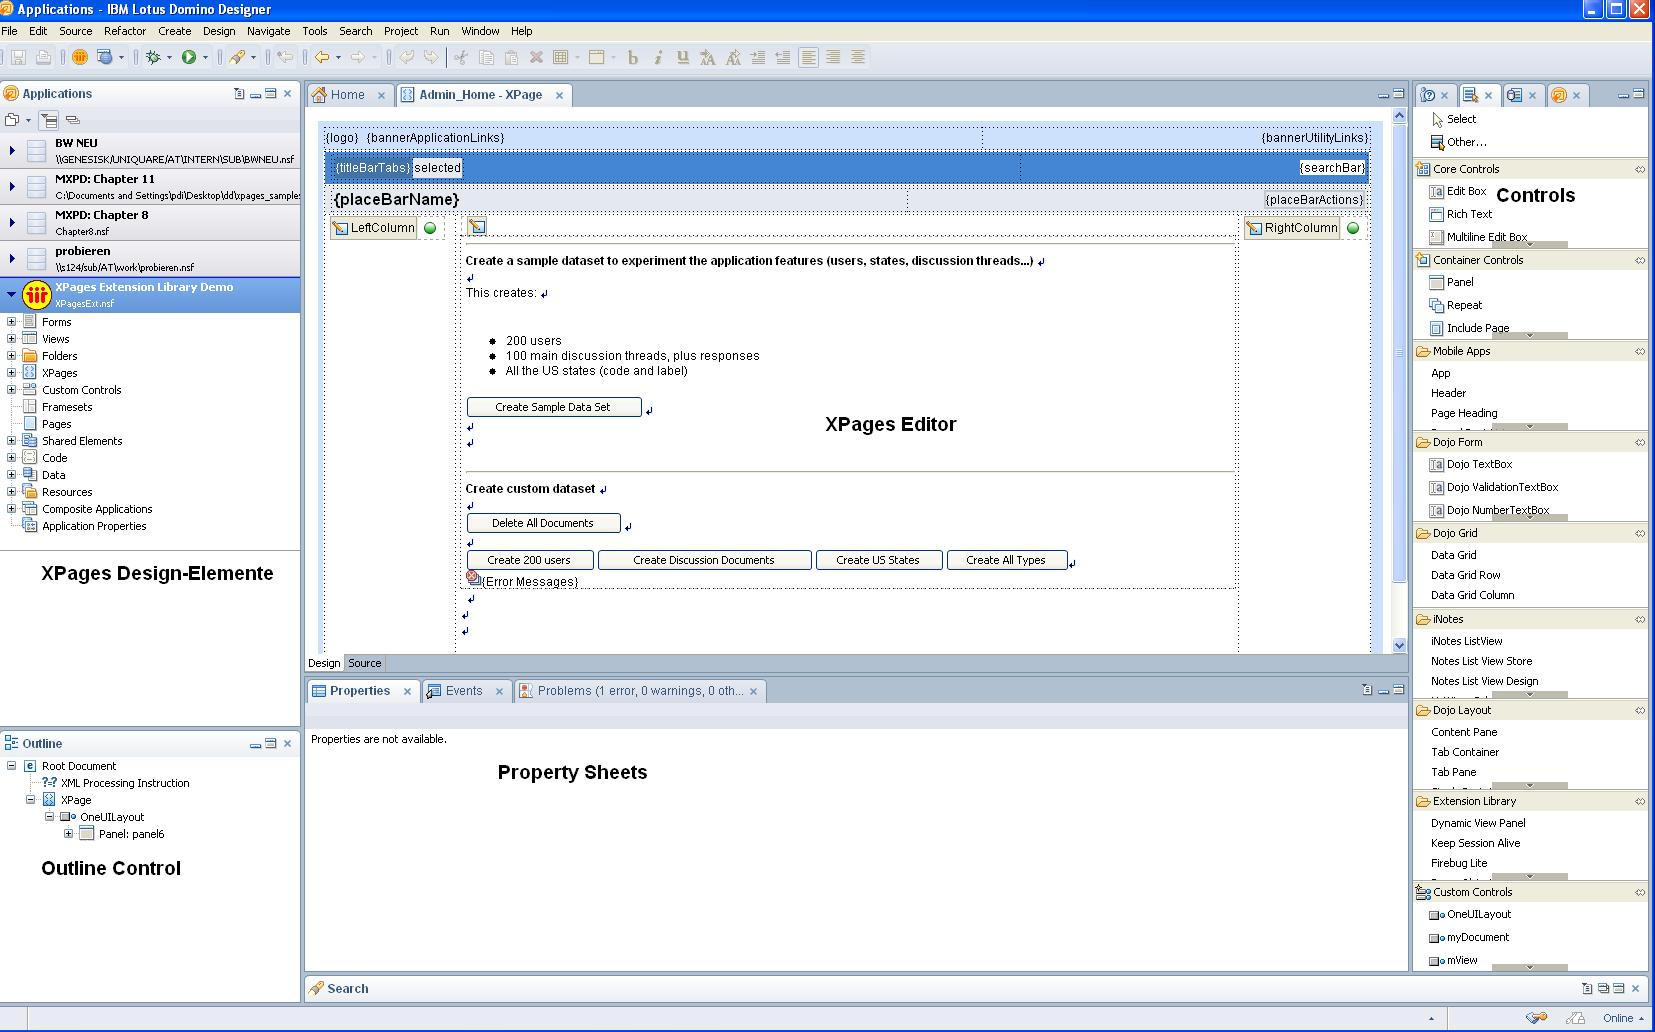
\includegraphics[scale=0.35]{pics/xpageseditor}}
    \caption[XPages Editor]{\label{FiG:XPages Editor}
	Verfügbare Tools im Designer 8.5}
\end{figure}
Abbildung 3.2 zeigt den Designer und wie dieser nach dem Erstellen eines Design-Elements, in diesem Fall einer XPage, verfügbar ist. 
Erst nach dem Erstellen einer XPage werden die Tools des Designers angezeigt und können auch verwendet werden.\newline
\newline Diese Tools sind:


\begin{itemize}
\item \textbf{XPages Editor,}
\item \textbf{Controls Palette,} 
\item \textbf{Outline Control,}
\item \textbf{Property Sheets,}
\item \textbf{XPages Design-Elemente.}
\end{itemize}
Die Informationen für die Beschreibung der Tools, wurden aus \cite{donelly} entnommen. 

\subsubsection{XPages Editor}
\label{sec:4designelemente}

Dieser Editor wurde speziell für XPages entworfen und unterstützt zwei Arten von Operationen:

\begin{enumerate}
\item \textbf{Default Mode:} In diesem Modus kann \textit{visual editing} vorgenommen werden. Das be-\linebreak deutet, dass mittels Doppelklick in den
 Editor,  
zum Beispiel direkt Text eingegeben \linebreak werden kann. Design-Elemente können mittels \textit{drag and drop} eingefügt werden. 
\item \textbf{Source Mode:} Eine XPage kann auch mittels Programmierung erstellt werden, da es sich um eine Extensible Markup Language (XML)-Datei 
handelt (Kapitel 3.2.4). 
In \linebreak diesem Modus können tags auf direkte Weise  eingegeben werden.\newline
\newline
\begin{graybox}
 \textit{Ein tag ist ein HTML Sprachelement, mit dem man unter Verwendung eines WWW-Browsers HTML Dokumente erstellen kann\cite{tag}. }
 \end{graybox} 
\end{enumerate}

\subsubsection{Controls Palette}
\label{sec:4designelemente}

Hier werden die verfügbaren \textit{controls}-Elemente des Designers abgebildet, nachdem die \textit{Extension Library} (Kapitel 3.4.1) eingebunden wurde.
In diesem Tool des Designers sind alle \textit{standard user interface controls} aufgelistet, welche zu einer XPage für die Entwicklung einer Applikation
hinzugefügt werden können.

\subsubsection{Outline Control}
\label{sec:4designelemente}

Um die Navigation innerhalb einer XPage zu erleichtern, wird eine Outline-Control zur \linebreak Verfügung gestellt.
Dieses Tool bildet eine hierarchische Darstellung der XPage ab, in welcher alle Elemente einer XPage aufgelistet sind.


\subsubsection{Property Sheets}
\label{sec:4designelemente}

In diesem Teil des Designers, kann für ein ausgewähltes Design-Element die spezifische \linebreak Konfiguration vorgenommen werden.\\ 
\newline
Dieser beinhaltet:
\begin{itemize}
\item \textbf{Properties:} Ermöglicht unter anderem die Namensgebung des Elements oder auch die Darstellung für das ausgewählte Element.
\item \textbf{Events:} Hier können events, wie zum Beispiel \textit{onClick}-Events, bestimmt werden. Ein \linebreak onClick-Event bestimmt welcher logische 
Schritt beim Anklicken eines Elements ausgeführt wird. Unter Verwendung dieser Events, kann die Logik der
Programmierung in diesem Tool des Designers vorgenommen werden. Das bedeutet, die Abfolge und \linebreak
Zusammenhänge der einzelnen XPages können an dieser Stelle festgelegt werden.
\item \textbf{Problems:} Hier werden Fehlermeldungen und Warnungen der aktuell geöffneten XPage angezeigt.
\end{itemize}

\subsubsection{XPages Design-Elemente}
\label{sec:4designelemente}

Hier sind alle verfügbaren Design-Elemente, welche der Domino Designer bereitstellt, angeführt. Die XPages Design-Elemente sind der Kernpunkt 
dieser Arbeit, darum werden diese im anschließenden Kapitel ausführlich behandelt.

%============================

\section{Details der XPages Design-Elemente}
\label{sec:4designelemente}

\subsection{Informationen zu Design-Elementen}
\label{sec:4designelemente}

Eine Datenbank ist der Aufbewahrungsort für die Daten und die Gestaltungselemente, die sich in einer Anwendung befinden. Design-Elemente sind die Bausteine
mit welchen eine \linebreak Anwendung erstellt wird.\\
\newline
Die hier angeführten Elemente sind nur ein Teil der verfügbaren Design-Elemente:
\begin{itemize}
\item Seiten,
\item Masken,
\item Felder,
\item Ansichten,
\item Agenten,
\item XPages,
\item Custom Controls. 
\end{itemize}

Um eine Applikation in Lotus Notes zu entwickeln, sind Design-Elemente zwingend notwendig. Es wurden für die Version 8.5 neue Design-Elemente, 
wie zum Beispiel XPages und Custom Controls, implementiert. Diese dienen im speziellen der weborientierten Darstellung.
Haupt-Design-Elemente wie \textit{forms} und \textit{views} sind bereits seit älteren Versionen implementiert und werden auch weiterhin unterstützt.
Die neu implementierten Elemente zielen auf die Entwicklung für Intra-und Internet. Es wird jedoch dem Entwickler einer Notes-Anwendung, mit
dem Schwerpunkt auf den Notes-Client, eine Reihe von Möglichkeiten geboten, um die Ent-\linebreak wicklung zu vereinfachen\cite{mann}.
Wie bereits in Kapitel 1.2 erwähnt, wird in dieser Arbeit ein \linebreak Template entwickelt, um Notes-Datenbanken mittels Browser-Zugriff zu verwalten.
In Folge werden die notwendigen Elemente im Einzelnen angeführt. In Abbildung 3.3 sind die \linebreak verfügbaren Design-Elemente des Domino Designers 8.5
ersichtlich.


\begin{figure}[H]
    \centerline{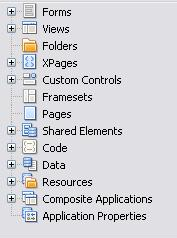
\includegraphics[scale=0.7]{pics/alleDesignelemente}}
    \caption[XPages Design-Elemente]{\label{FiG:XPages Design-Elemente }
	Design-Elemente }
\end{figure}

%============================

\subsection{Masken (Forms)}
\label{sec:4designelemente}

Masken sind elektronische Formulare, welche f\"ur die Erstellung von Dokumenten \"uber das graphical user interface (GUI) verwendet werden k\"onnen. 
Notes-Dokumente werden aus Masken erstellt, die von einem Anwendungsentwickler gestaltet werden.
Eine dieser Masken besteht in der Regel aus mehreren Felddefinitionen. 
In diesen ist die Datenstruktur eines bestimmten Dokumenttyps festlegt. Des weiteren kann eine Maske Formatierungsmerkmale
wie zum Beispiel Text, Grafiken und Tabellen beinhalten. Es können auch fortgeschrittene Features, wie OLE-Objekte (nur im Notes Client) und Java-Applets
in Masken enthalten sein.
Die Notwendigkeit von Masken liegt darin, da sie der häufigste Weg sind, um Inhalte einer Domino-Datenbank zu erstellen.\newline
Masken dienen als \textit{Schablonen für Dokumente}.
Bei der Erstellung einer Maske, wird die interne Struktur des Dokumentes nach der Schablone festgelegt. Realisiert wird diese Strukturierung
unter der Verwendung von Feldern. Domino erstellt intern eine Verknüpfung zwischen dem erstellten Dokument und der gewählten Maske. 
Wird ein Dokument aufgerufen, wird dieses automatisch im Rahmen der jeweiligen Maske dargestellt (Abbildung 3.4). Weiters kann somit auch die 
Formatierung eines Dokumentes beeinflusst werden\cite{knaepper}.

\begin{figure}[H]
    \centerline{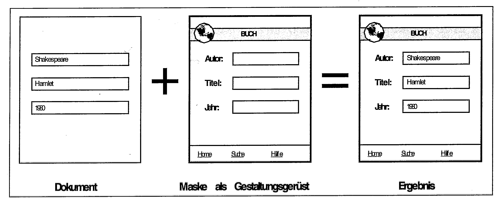
\includegraphics[scale=0.7]{pics/maskeGestaltung.png}}
    \caption[Maskengerüst]{\label{FiG:Maskengerüst }
	Masken-Gestaltungsgerüst\cite{knaepper}}
\end{figure}

Es gibt die Möglichkeit eine Maske von Grund auf neu zu erstellen, da es aber für die bestehenden Datenbanken bereits Masken gibt, wird
dies nicht weiter behandelt.

\begin{figure}[H]
    \centerline{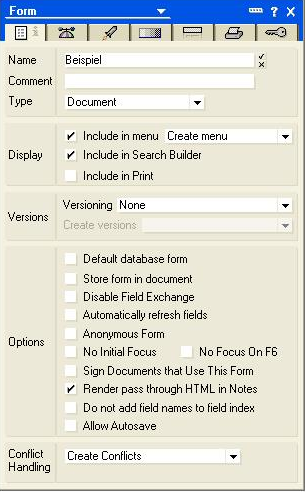
\includegraphics[scale=0.5]{pics/maske}}
    \caption[Eigenschafts-Fenster für Masken]{\label{FiG:form_Control }
	Eigenschaften einer Maske}
\end{figure}

Die Abbildung 3.5 zeigt das Eigenschafts-Fenster einer Maske. In diesem Bedienfenster können unter anderem der Namen und das Verhalten
einer Maske festgelegt werden. Für eine detailliertere Beschreibung wird auf die Fachliteratur verwiesen.

%============================

\subsection{Ansichten (Views)}
\label{sec:4designelemente}

Das Ziel eines Entwicklers ist es, dem Anwender genau \textit{die} Information zu liefern, welche er benötigt bzw. erwartet. 
Für die Darstellung von Dokumenten sind Ansichten notwendig. Eine solche besteht aus Spalten, in welchen die Werte aus
Dokumenten oder berechnete Werte angezeigt werden. 
Die berücksichtigten Dokumente werden über eine Selektionsformel ausgewählt.\newline 

\begin{figure}[H]
    \centerline{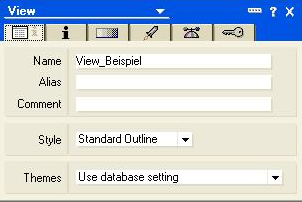
\includegraphics[scale=0.7]{pics/view}}
    \caption[Eigenschafts-Fenster für Ansichten]{\label{FiG:View_Control }
	Eigenschaften einer Ansicht}
\end{figure}
Im Eigenschaftsfenster einer Ansicht werden die \textit{eigentlichen} Einstellungen vorgenommen. 
Neben den Basic-Konfigurationen wie der Namensgebung,
können hier die Ansichtsoptionen, die Formatierung und eine Reihe weiterer Einstellungen einer Ansicht festgelegt werden.\\ 

Vor der Version 8.5 des Designers war eine teilweise, separate Programmierung für die Darstellung im Web oder im Notes-Client notwendig. 
Um dies zu erreichen, konnten Masken und Ansichten optional, freigegeben oder verborgen werden. Somit ergaben sich unabhängige Programmierungen für die 
Benutzung durch Client und Browser, jedoch stieg damit auch der Programmieraufwand.
%An dieser Stelle ist keine nähere Betrachtung der Ansichten von Nöten, da die Ansichten bereits erstellt wurden.\newline


%============================

\subsection{XPages}
\label{sec:4designelemente} 

Wie in diesem Kapitel bereits erläutert, ist jedes Design-Element für eine spezielle Aufgabe zugeschnitten.
\textit{Masken} sind notwendig um Notes-Dokumente zu erstellen und zu bearbeiten, während \textit{Ansichten} für die Darstellung 
der Dokumente benötigt werden.
Im Grunde genommen sind XPages, statische Seiten die im Domino-Designer definiert werden.
Bis zur Version 8.5 musste f\"ur die Darstellung im Web oder Notes-Client in der Programmierung R\"ucksicht auf die gew\"unschte Art der Darstellung
 (Web oder Client) genommen werden. Es wurde meist eine unterschiedliche Version f\"ur das Web und den Client erstellt.\newline
XPages ermöglichen es, mit einer einzigen Implementierung eine Darstellung und Benutzung im Notes-Client \textit{und} im Web.
Wenn eine XPage über einen Browser aufgerufen wird, beginnt der Java Server Faces (JSF\footnote{Java Server Faces (JSF) ist eine Technologie zur Entwicklung von
Webanwendungen\cite{marinschek}.})-Lebenszyklus\cite{donelly}.\newline


Eine XPage ist ein speziell entwickeltes leistungsstarkes Notes Design-Element, für die \linebreak Darstellung von Notes-Datenbanken im Web
2.0 sowie für den Notes-Client. XPages bieten die Besonderheit, dass die Darstellung im
Web und im Client, sowie auch die Bedienung,\linebreak identisch sind\cite{donelly}.

%\footnote{Definition zu Web 2.0\cite{messerschmidt}} 
\vspace{0.5cm}

\subsubsection{Dateiformat einer XPage}
\label{sec:4designelemente}

XPages und auch Custom Controls (Kapitel 3.2.5) verwenden XML als Dateiformat. Die \linebreak Informationen für HTML und XML
wurden sofern nicht anders angegeben,
aus den Lehrveranstaltungsunterlagen zu Webengineering, von FH-Prof. Univ.-Doz. Dr. Elke Hochmüller entnommen.
XML dient der Strukturierung, der Speicherung und dem Austausch von Daten.\\

 Das Wesen von XML:
\begin{itemize}
\item Daten können mit XML beschrieben werden.
\item XML ist ein hardware-, software- und applikationsunabhängiges Datenformat.
\item XML ermöglicht den Datenaustausch zwischen inkompatiblen Systemen. 
\item XML ist eine Auszeichnungssprache und vergleichbar mit HTML. 
\end{itemize}
HTML ist die am weitesten verbreitete Strukturierungssprache. Trotz Parallelen zu XML, \linebreak werden diese klar unterschieden.\\
\newline
Die markantesten Unterschiede sind:
\begin{itemize}
\item Dokumente müssen korrekt genestet (well formed) sein.
\item Dokumente müssen ein schließendes \textit{tag} besitzen.
\end{itemize}
Diese beiden Sprachen besitzen eine unterschiedliche Zielsetzung, sie stehen in keiner Konkurrenz zueinander.
Mit XML werden Daten beschrieben, HTML ermöglicht die Darstellung von Daten.
XML tags werden vom Anwender selbst, in der Document Type Definition (DTD) definiert.


\subsubsection{XPages und XML Syntax}
\label{sec:4designelemente}

In XPages wird XML benutzt, um ein erklärendes Programmierungs-Modell zu definieren. Es wird rein die Darstellung definiert, ohne sich
darum kümmern zu müssen, wie diese \linebreak tatsächlich geschieht. Ziel ist es, dem Entwickler mit vorgefertigten Design-Elementen \linebreak 
dahingehend zu unterstützen,
dass mit möglichst wenig Programmieraufwand eine \linebreak Applikation erstellt werden kann. 
Es ist nicht möglich, komplett ohne Codierung eine Applikation zu erstellen\cite{donelly}.\\
\newline
Jedoch werden vom Domino-Designer folgende Anwendungsmöglichkeiten, ohne Programmieraufwand, bereitgestellt:
\begin{itemize}
\item Erstellen des \textit{user interfaces}\footnote{User interface ist die Darstellung, welche dem Benutzer zur Interaktion mit dem System bereitgestellt wird.} 
für eine Applikation.
\item Definieren der Daten, welche geändert und dargestellt werden.
\item Definieren der Logik, welche bei Anfragen an die Datenbank ausgeführt werden soll. 
\end{itemize}

Hierfür werden tags benötigt, diese sind die Grundbausteine, um eine Anwendung \linebreak darzustellen. Jeder dieser tags entspricht einem Kontrollelement
für den Benutzer, einer \linebreak Datenquelle, der vordefinierten Logik, oder einer Eigenschaft die von einer dieser Komponenten genutzt wird.
Es ergibt sich eine klar definierte Interaktion zwischen der Benutzeroberfläche, den Daten und der logischen Komponenten.\newline
Jede XPage ist ein XML Dokument und muss einen \textit{root-tag} besitzen. 
Der root-tag einer XPage wird beim Erstellen einer neuen XPage automatisch generiert und ist im Source-View \linebreak (Abbildung 3.7) ersichtlich. \newline

\begin{figure}[H]
    \centerline{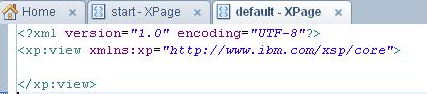
\includegraphics[scale=0.7]{pics/root-tag}}
    \caption[Root Element einer XPage]{\label{FiG:root-tag }
	root-tag}
\end{figure}


Für weitere Informationen zu diesem Kapitel wird auf \cite{donelly} verwiesen. 

%============================
 
\subsection{Custom Controls}
\label{sec:4designelemente} 
 
Das letzte Designelement, welches in dieser Arbeit beschrieben wird, sind Custom Controls. Als Quelle dieses Kapitels diente \cite{donelly}.
Das grundlegende Konzept, das hinter diesem Design-Element steckt, sind Programmbausteine. Custom Controls sind die Bausteine einer XPage.

\subsubsection{Divide and Conquer} 
\label{sec:4designelemente} 
Mit Custom Controls wird ein Divide and Conquer Prinzip verfolgt. Dieses Prinzip baut \linebreak darauf, eine Datenbank-Anwendung aus kleineren
 Programmbausteinen zusammenzusetzen. Ein \textit{Custom Control Block} besteht aus Daten und dem Layout.
Diese wiederverwendbaren Bausteine können mittels drag and drop in die bestehenden XPages eingefügt werden. Wie auch das Design-Element XPages
werden beim Entwerfen von Custom Controls, XML-tags generiert.
Dies bringt den Vorteil mit sich, dass kleinere Bausteine schneller entwickelt und beliebig zusammengesetzt werden können. 
Der größte Vorteil von diesen Bausteinen ist \linebreak ihre vielseitige Einsatzmöglichkeit. So können diese mehrmals in die selbe XPage, innerhalb 
der \linebreak selben
Anwendung beliebig oft oder in andere Anwendungen eingefügt werden. 
Eine \linebreak Besonderheit dabei ist, dass der Geltungsbereich von eingebetteten Custom Controls in \linebreak XPages, bei jedem Einfügen, 
\textit{eindeutig instantiiert}
 wird.
\newline


Um ein Custom Control zu erstellen, gibt es wie in Kapitel 3.1.1 erwähnt, zwei Möglichkeiten.
Wird ein Custom Control im Default Mode erstellt, erfolgt dies nach dem WYSIWYG Prinzip. 
%WYSIWYG ist ein Akronym und steht für What-You-See-Is-What-You-Get. Im Bereich der Webentwicklung ist ein WYSIWYG-Programm 
%ein Werkzeug, bei welchem die Darstellung während der Bearbeitung und der späteren Anzeige im Browser exakt übereinstimmen\cite{jendryschik}.


\subsubsection{Verwendungsmöglichkeiten von Custom Controls} 
\label{sec:4designelemente} 

Dieses Design-Element kann auf zwei verschiedene Arten verwendet werden:\\
\newline
%Diese Möglichkeiten sind:
\begin{itemize}
\item Ein Custom Control kann als \textit{Aggregate Container} benutzt werden. Für diese Variante wurde für dieses Design-
Element entwickelt.
 %Entwicklung, welcher hinter diesem  steht. 
Wie schon im Abschnitt Divide and Conquer erläutert, können die erstellten Custom Controls beliebig oft in eine Anwendung und auch in andere Datenbank-
Anwendungen eingebunden werden. Die Entwicklung eines Custom Control-Elementes ist nur einmal notwendig. Danach kann das erstellte Element beliebig oft
wieder verwendet  werden. 
\item Eine andere Verwendungsmöglichkeit ist das Benutzen eines Custom Controls als \textit{Layout Container}. Hierbei können innerhalb eines Custom Controls, Design-Elemente für das Layout verschachtelt werden. Es wird somit ein Design-Template erstellt.
\end{itemize}

Verbindet der Entwickler beide möglichen Varianten, kann eine Datenbank Anwendung mit wenig Zeitaufwand erstellt werden. Für weitere Informationen zu 
diesem Design-Element wird auf \cite{donelly} verwiesen.



%============================

\section{Unterstützte Programmiersprachen}
\label{sec:4designelemente}

\subsection{Formelsprache}
\label{sec:4designelemente}

Signifikant für die Formelsprache in Lotus Notes sind @-Befehle und -Funktionen. Diese Befehle und Funktionen können für alle Bereiche, in denen
Formeln zur Programmierung zur Verfügung stehen, über Referenzlisten ausgewählt werden. Der Editor unterstützt für die \linebreak Formelsprache die farbliche
Darstellung zur Unterscheidung der einzelnen Codesegmente. Wird ein Fehler erkannt, wird dieser Code-Teil in Rot dargestellt. Weiters wird in der Statuszeile
des Editorfensters eine Beschreibung des gefundenen Fehlers abgebildet\cite{mann}.\\
In der Version 8.5 des Designers, ist für @-Funktionen eine Bibliothek hinterlegt. Diese \linebreak Funktionen der Bibliothek, sind eine Sammlung von JavaScript
Methoden. Die Methoden \linebreak bieten häufig in Notes benutzte Operationen, wie zum Beispiel der Rückgabewert des Autors des aktuellen Dokumentes\cite{donelly}.\newline 
Ein Beispiel für die Formelsprache in Notes finden sie in Folge.
Eine Selektionsformel gibt an, aus welchen Dokumenten eine Darstellung, beziehungsweise, wie die Darstellung ausgeführt werden soll.\\
Eine in der Formelsprache implementierte Selektionsformel beginnt \textit{immer} mit dem Schlüsselwort \textit{select}. 
Mit der Selektionsformel $ Select @ All$ werden alle Dokumente einer Datenbank in dieser Ansicht dargestellt. 
Da es aber nicht das Ziel ist alle Dokumente anzuzeigen, kann mit spezifischen Formeln, auch nur bestimmte Feldinhalte ausgegeben werden.\\
Als Bedingung wird eine Maske angegeben, wie in diesem Beispiel ersichtlich:
\begin{equation}
Select (form=``Beispiel'')
\end{equation} 

In diesem Fall werden nur Dokumente mit einem bestimmten Feldinhalt (aus der Maske Beispiel) ausgegeben.
Des weiteren ist es auch möglich, mehrere Dokumente als Bedingung anzuführen. \\
Um dies zu erreichen, gibt man eine zusätzliche Maske wie folgt an:
\begin{equation}
 Select (form=``Beispiel'':``NeueMaske'')
\end{equation}


\subsection{LotusScript}
\label{sec:4designelemente}

Die Programmiersprache mit der höchsten Integration in Lotus Notes ist LotusScript. LotusScript ist voll in die IDE integriert.  
Es stehen für alle LotusScript -Befehle und -Funktionen Referenzlisten zur Verfügung.
Wird ein Ereignis ausgewählt, stellt Lotus Notes automatisch alle Bestandteile der Script-Routine zur Verfügung.
Der Sourcecode dieser Sprache wird Events zugeordnet, deshalb ist es nicht möglich den gesamten Code, wie in anderen Editoren, einzusehen.
Ziel dieser Sprache ist es, nur kleine überschaubare Einheiten des Source-Codes einzusehen, da die Wartung und das Handling vereinfacht werden 
soll\cite{mann}. 

\subsection{JavaScript}
\label{sec:4designelemente}

JavaScript steht für den Zugriff einer Datenbank über einen Web Browser. Hierfür wurde \linebreak speziell für JavaScript, eine Adaptierung des W3C Document
Object Model erstellt.
Wie in Abschnitt 3.3.1 bereits erwähnt, ermöglichen XPages dem Entwickler die Benutzung von Java- Script. Unter Verwendung dieser
Programmiersprache, kann eine eigene Logik in eine \linebreak Anwendung implementiert werden\cite{donelly}.\\ 
Um diese Logik einzubinden gibt es die Möglichkeit einer \textit{ serverseitigen-} oder \textit{ clientseitigen-}Programmierung.
Abhängig von der gewählten \textit{Seite}, von welcher das Script aufgerufen wird, gibt es Unterschiede:
\begin{itemize}
\item \textbf{Object Model:} Dieses Model wird für die Darstellung der XPage benutzt. 
\item \textbf{Global objects:} Eingebettete Objekte, welche referenziert werden können.
\item \textbf{System libraries:} Bibliothek mit Klassen, welche benutzt werden können.
\end{itemize}

\subsubsection{Serverseitige Programmierung}
\label{javascript}

XPages bieten eigene Object Models um JavaScript zu verwenden. Diese Object Models sind eine Kombination aus JSF Object models, Document Object
models und einigen Objekten \linebreak welche die Entwicklung vereinfachen sollen. Das Document Object Model ist eine Schnittstelle, mit welcher auf eine
Bibliothek zugegriffen werden kann.
Diese Bibliothek enthält eine \linebreak Sammlung von Klassen und Methoden, welche dafür benutzt werden können, um ein XML Dokument zu erstellen oder zu
verändern\cite{donelly}.\\
\newline
Mit serverseitiger Programmierung können:
\begin{itemize}
\item Design-Elemente manipuliert werden,
\item Informationen zu Anfragen ausgelesen werden,
\item Interaktionen mit dem laufenden Prozess durchgeführt werden,
\item Auslesen von Informationen zum aktuellen Status der Anwendung.
\end{itemize}

Auf die \textit{global objects} und \textit{System Libraries} kann über die Property Sheets (3.1.4), im Events Tab zugegriffen werden. 


\subsubsection{Clientseitige Programmierung}
\label{javascript}

Die Entwicklung von clientseitigem JavaScript unter XPages, ist dieselbe wie die einer \linebreak Webanwendung.\\
\newline
Es müssen dabei folgende Faktoren beachtet werden:
\begin{itemize}
\item Control ID versus Client ID,
\item Einbinden der Server Daten im clientseitigen JavaScript,
\item Hinzufügen der Server-und Clientseitigen Logik für dasselbe Ereignis.
\end{itemize}
\vspace{0.5cm}


\textbf{Control ID versus Client ID: } Die ID, welche in der XPage ausgezeichnet wird, entspricht nicht derselben ID, welche vom dazugehörigem Element
in der HTML DOM erzeugt wird. Dies geschieht aufgrund dessen, weil die JSF Funktionseinheit eine unterschiedliche ID erzeugt, welche für die allgemeine
Auszeichnung gültig ist. \newline
\newline


\textbf{Einbinden der Server Daten im clientseitigen JavaScript: } Dieser Schritt muss vorgenommen werden, um das Ergebnis einer serverseitigen Berechnung,
 im clientseitigem Script zu verwenden.\newline
 \newline



\textbf{Server-und clientseitigen Logik für dasselbe Ereignis: } Es kann eine server- und clientseitige Logik, welche demselben Ereignis
zugeordnet ist, hinzugefügt werden.


\subsection{Java}
\label{sec:4designelemente}

Java ist eine plattformunabhängige objektorientierte Programmiersprache. Diese Sprache und das DOM sind kompatibel.
Das bedeutet, dass Java auf die Dokumente von Domino zugreifen kann. Es können zum Beispiel Daten ausgelesen, oder verändert werden.\\
\newline
Es gibt zwei Möglichkeiten Java-Code einzubinden:
\begin{itemize}
\item inside Java,
\item outside Java.
\end{itemize} 

\par Wird inside Java für eine Anwendung verwendet, kann dies zum Beispiel für die Erstellung von Agenten benutzt werden. Agenten sind Programme, die
eine Reihe automatisierter und zeitkritischer Aufgaben ausführen\cite{ebel}.
Mit Java outside hingegen, ist es möglich Anwendungen zu schreiben die auf eine Domino Datenbank beeinflussend wirken. 
Weiters wird Java dazu benutzt um mit serverseitigen Anwendungen, den Servlets, zu interagieren\cite{mccoy}. 



%==================================================================================================
\section{Template}

In diesem Kapitel werden Konfigurationen und Vorkommnisse dokumentiert, welche im \linebreak Laufe der Template-Entwicklung aufgetreten sind. 
Um Design-Elemente wie XPages \linebreak und Custom Controls sowie die erweiterten Funktionalitäten dieser Elemente nutzen zu können, mussten
erweitere Konfiguration vorgenommen werden. 

%========================
\subsection{Anforderungen}
\label{sec:6template}
Um weitere Gestaltungs-und Funktions-Elemente zu verwenden, muss zu Beginn einer Entwicklung eine weitere Konfiguration vorgenommen werden.
In dieser Konfiguration wird eine erweiterte Bibliothek namens \textit{XPages Extension Library} eingebunden.
Diese Bibliothek wird als Open-Source-Project angeboten\footnote{http://extlib.openntf.org} und kann kostenfrei heruntergeladen werden.\newline
Unter Open-Source versteht sich, dass der Quellcode einer Software dem Anwender zur \linebreak Verfügung gestellt wird.
Es existiert eine Dokumentation, welche den korrekten Weg beschreibt um die Bibliothek einzubinden. Weiters beinhaltet diese Dokumentation 
eine Auflistung
der verfügbaren Control Design-Elemente. 
Für den exakten Ablauf der Installation wird an dieser Stelle auf diese Dokumentation verwiesen.
\vspace{0.5cm}

\vspace{0.3cm}


Hier werden die durchzuführenden Schritte angeführt:

\begin{enumerate}
\item Bibliothek in Domino-Designer einbinden,
\item Bibliothek auf Server installieren,
\item Installieren und ausführen der \textit{Demo-Applikation}.
\end{enumerate}

\vspace{0.5cm}

\begin{graybox}
\textbf{\textit{Wichtiger Hinweis:}} Es gilt den in der Dokumentation angegeben Pfad \textbf{unbedingt} einzuhalten, ansonsten ist die Nutzung der External
 Library nicht möglich.
\end{graybox}

\vspace{0.5cm}
%========================
\subsection{Virtueller Server}
\label{sec:6template}

Um sicherzustellen, dass es nicht durch etwaige Firewalls zu einer Einschränkung der \linebreak Funktionalität führen kann, wurde ein virtueller Server angelegt.
Dies sollte weiters dem Zweck dienen, dass die Tests der Implementierung, sollte es zu Fehlern kommen, nicht zu Lasten eines aktiven Servers gehen.
Somit wurde sichergestellt, dass die Entwicklung in einer abgekapselten Umgebung durchgeführt wurde.

%========================
\subsection{Template-Realisierung}
\label{sec:6template}

%In der Abbildung 3.8 ist die Anwendung, wie es in einem Webbrowser dargestellt wird, ersichtlich.

\begin{figure}[H]
    \centerline{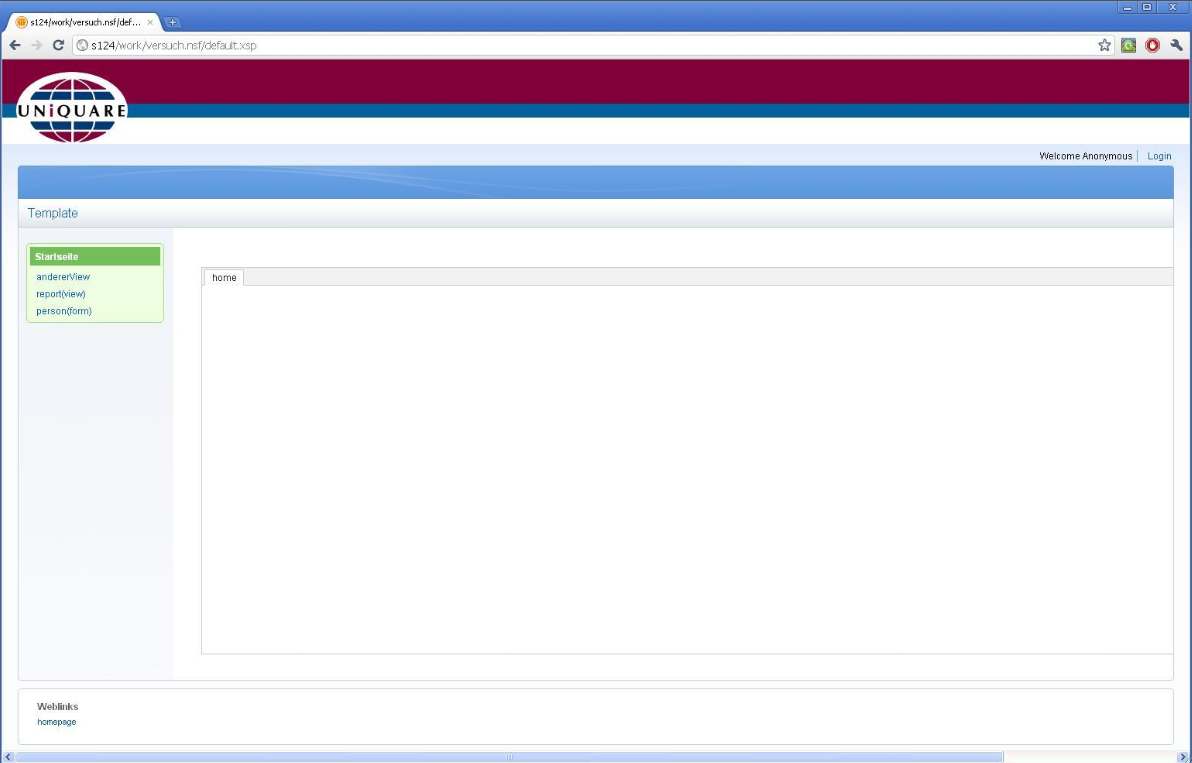
\includegraphics[scale=0.3]{pics/template_chrome}}
    \caption[Template in Browser]{\label{FiG:Template in Browser }
	Template in Browser}
\end{figure} 


%Wie in Kapitel 3.4.2 erwähnt, befindet sich die erstellte Anwendung auf einem virtuellen Server. 
Diese Anwendung kann von jedem berechtigten Notes-Client
innerhalb der erlaubten \linebreak Domäne, sowie auch über einen Webbrowser aufgerufen und ausgeführt werden. In Abbildung 3.8 ist die erstellte Anwendung 
in ihrer Startansicht ersichtlich.\newline 

\subsubsection{Aufbau des Templates}
\label{sec:6template}

Für jeden Link auf der dargestellten Seite und auch das Layout, sind XPages in Verbindung mit Custom Controls erstellt worden.
Für diese Anwendung wurden vier XPages implementiert. Jede dieser XPages ist für eine unterschiedliche Verwendung als Vorlage zu sehen.\\
\newline
Diese XPages sind:
\begin{itemize}
\item \textbf{default.xsp} - Darstellung der Startseite.
\item\textbf{ another.xsp} - Zeigt einen mit DOJO erstellten Container mit der Darstellung einer Ansicht\cite{steyer}.
\item \textbf{report.xsp} - Ist eine XPage mit implementierter Ansicht.
\item \textbf{person.xsp} - Gibt eine editierbare Darstellung einer Maske wieder.
\end{itemize}
Um ein Auswahlmenü zu erstellen wurde eine Stilvorlage, welches als Custom Control in der Extension Library verfügbar ist, bereitgestellt und 
eingefügt. Diese kann der Entwickler nach Vorgaben gestalten. Das heißt das Layout wird durch ein Custom Control bestimmt und die logischen
Verknüpfungen werden in einem implementierten File vorgegeben. In dieser Stilvorlage, unter Property File, werden die XPages mit den 
dargestellten Titeln der Links angegeben (Abbildung 3.9). 
\begin{figure}[H]
    \centerline{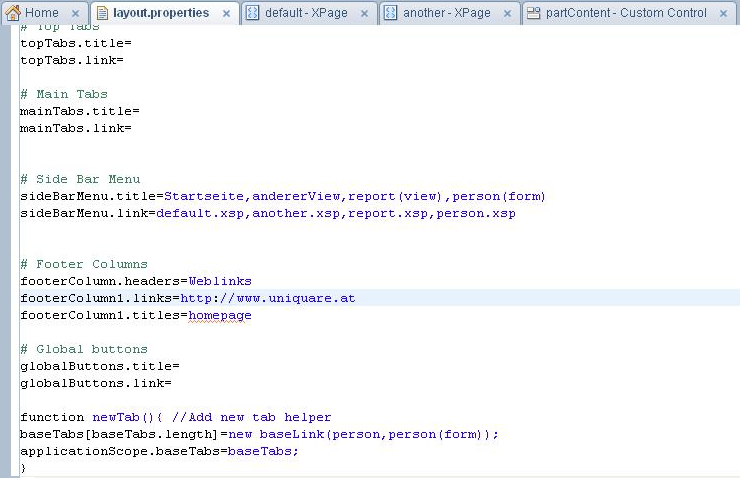
\includegraphics[scale=0.4]{pics/layoutproperties}}
    \caption[Haupt-Menü der Anwendung]{\label{FiG:Haupt-Menü der Anwendung}
	Property File }
\end{figure}
Jede der im Auswahlmenü verfügbaren XPages wird als Link dargestellt. Wird ein Link ausgewählt, wird die jeweilige XPage in den Browser oder Notes-Client
geladen und kann bearbeitet oder gelesen werden.\newline
Wie in Kapitel 3.1 beschrieben, wird eine XPage in einem Editor zusammengestellt. Eine \linebreak mögliche Zusammensetzung wird in Abbildung 3.10 
anhand der default.xsp des erstellten \linebreak Templates, abgebildet.
\begin{figure}[H]
    \centerline{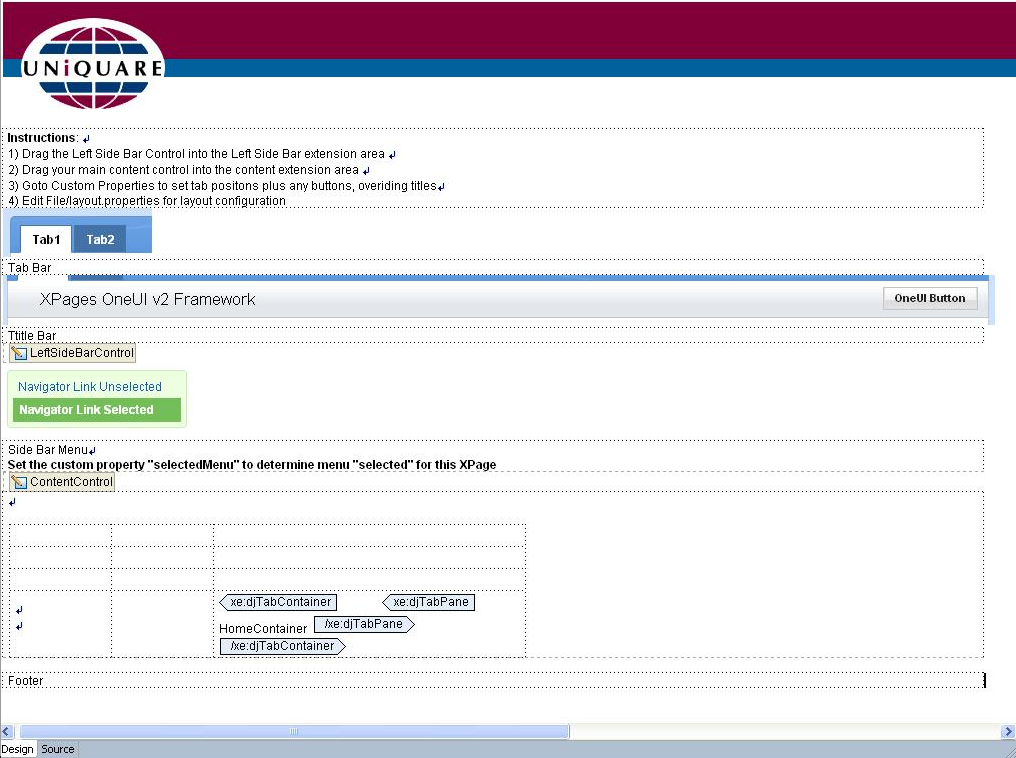
\includegraphics[scale=0.3]{pics/xpagesineditor}}
    \caption[XPages Editor mit default.xsp ]{\label{FiG:XPages Editor mit default.xsp}
	WYSIWYG-Editor}
\end{figure}
Unter Verwendung des Dojo Toolkits wurde bereits die Darstellung eines Containers \linebreak realisiert. Das Dojo Toolkit ist eine freie JavaScript 
Bibliothek für die Entwicklung von \linebreak Asynchronous Javascript and XML (AJAX) oder JavaScript basierenden Anwendungen. Wird innerhalb dieses
Containers ein Datensatz ausgewählt, öffnet sich ein neuer Tab innerhalb des Containers. Um dies zu erreichen, muss eine serverseitige Programmierung
vorgenommen \linebreak werden.
Die Realisierung ist in  Abbildung 3.11 ersichtlich.
\newline


AJAX beschreibt eine standardisierte Vorgehensweise, um eine Reaktion einer Webseite in Echtzeit gewährleisten zu 
können, obwohl neue Daten vom Web-Server abgefragt werden. \linebreak Anstatt einer vollständigen Webseite, wird eine Datenanfrage für einen bestimmten Teil abgerufen,
und dieser in die bereits zuvor geladene Abfrage eingebaut\cite{steyer}.

\begin{figure}[H]
    \centerline{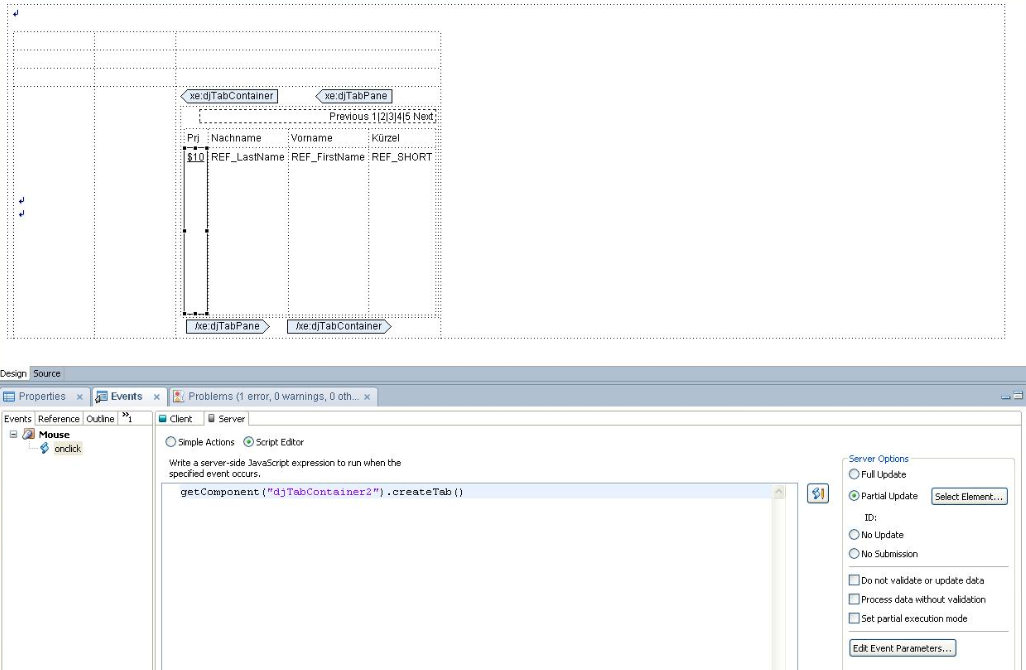
\includegraphics[scale=0.4]{pics/dojoContainer}}
    \caption[Dojo Container ]{\label{FiG:Dojo Container}
	Dojo Tab Container}
\end{figure} 



%========================
\subsection{Fehlermeldungen}
\label{sec:6template}

Um sich den Vorgang einer Entwicklung von Grund auf zu erleichtern, empfiehlt es sich bestehende Templates zu verwenden.
Wird ein vorgefertigtes Template verwendet, können Fehler wie zum Beispiel \textit{Unexpected runtime error} auftreten.
\newline
Es wird ein Beispiel angeführt, welches bei der Entwicklung aufgetreten ist. Zugleich wird auch der Lösungsweg beschrieben.
Wird ein Template verwendet, muss beim Verwenden von \linebreak diesem, auf die Verschlüsselung geachtet werden. Hierfür muss im Notes-Client, unter
\textit{\linebreak properties - Encryption Settings} die lokale Verschlüsselung \textit{deaktiviert} werden. Wird dies nicht beachtet, kann außer dem Ersteller 
niemand auf die Datenbank zugreifen. Ist die \linebreak Verschlüsselung konfiguriert worden, muss die Datenbank auf dem Server
gespeichert werden.
\vspace{0.5cm}
\begin{figure}[H]
    \centerline{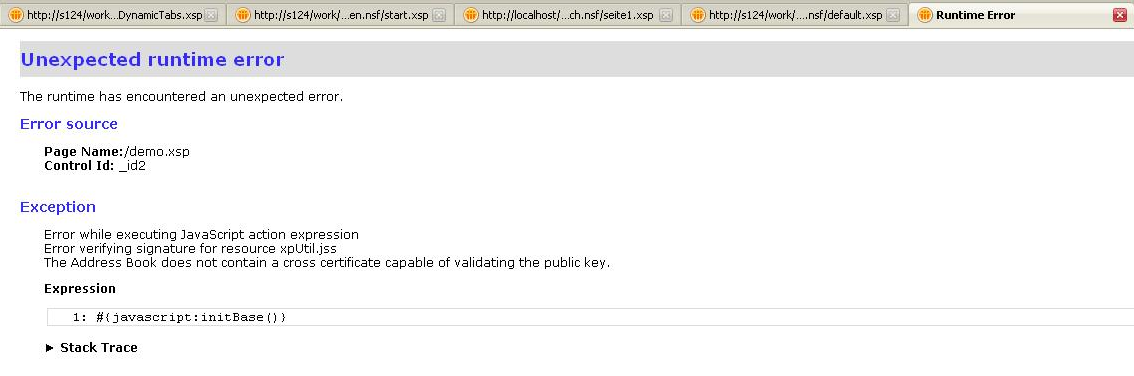
\includegraphics[scale=0.4]{pics/runtimeError}}
    \caption[Fehlermeldung - Unexpected runtime error]{\label{FiG:Unexpected-Runtime-Error }
	Runtime error }
\end{figure} 

In Abbildung 3.12 ist eine Fehlermeldung ersichtlich. Dieser Fehler erscheint wenn, die \linebreak Signaturen der Datenbank nicht übereinstimmen. 
Die Signatur des
Erstellers und des \linebreak Benutzers sind nicht dieselbe. Mit dem Ergebnis, dass der Server die Datenbank nicht im Browser darstellen kann. 
\\
\newline
Um diesen Konflikt zu vermeiden, sollten folgende Schritte eingehalten werden:
\begin{itemize}
\item Sollten im Designer bereits Design-Elemente geöffnet sein, müssen diese \linebreak geschlossen werden.
\item Ändern der Signatur im Domino Administrator-Client. 

\end{itemize}
\vspace{0.3cm}
Es besteht auch die Möglichkeit, jedes Designelement einzeln zu \textit{signen}.% von dieser Möglichkeit ist jedoch abzuraten. 

%==================================================================================================
